\cxset{style51/.style={
 chapter opening=any,
 name=CHAPTER,
 numbering=arabic,%change to WORDS
 number font-size=Large,
 number font-weight=normal,
 number font-family=rmfamily,
 number before=\kern0.5em,
 number dot=,
 number position=rightname,
 number border-width=0pt,
 number padding-bottom=0pt,
 number border-style=none,
 chapter border-width=0pt,
 %chapter name
 chapter color=black!80,
 chapter font-size= Large,
 chapter font-weight=normalfont,
 chapter font-family=sffamily,
 chapter before=,
 chapter spaceout=soul,
 number after=,
 chapter after=,
 chapter margin left=2cm,
 number color=black!80,
 chapter padding=0pt,
 %chapter title
 chapter title width=0.8\textwidth,
 title font-family=normalfont,
 title font-color=black!80,
 title font-weight=,
 title font-size=huge,
 chapter title align=none,
 chapter title text-align=left,
 title margin-left=2cm,
 title before=,
 title after=,
 title beforeskip=,
 title afterskip=,
 author block=false,
 section font-size=\Large,
 section font-weight=bfseries,
 section indent=0pt,
 epigraph width=\dimexpr(\textwidth-2cm)\relax,
 epigraph align=left,
 section font-weight=\normalfont,
 header style=empty}}

\cxset{style51}

\chapter[Template 51]{The Secret Meetings\\ of the Executive Committee\\ of the National Security Council\\  Style Fifty One}

\par
\bigskip
\hspace*{2cm}\begin{minipage}{0.7\textwidth}
                     \textbf{\sffamily Tuesday, October 16, 11:50 \textsc{a.m}, Cabinet Room}\par
                 ``How do you know this is a medium-range ballistic missile?''\\President John F. Kennedy.
\end{minipage}
\bigskip

\noindent This is an unusual book with a rather unique style. The vertical rule is simple and breaks the monotony of a book that is heavy on text.
\begin{figure}[ht]
\fbox{%
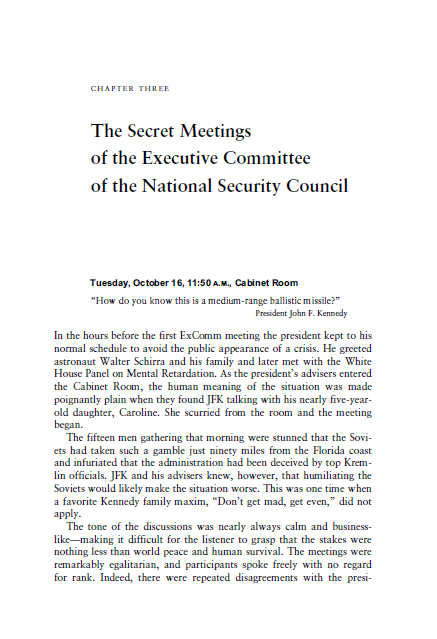
\includegraphics[width=0.48\textwidth]{./chapters/chapter51.png}\hfill
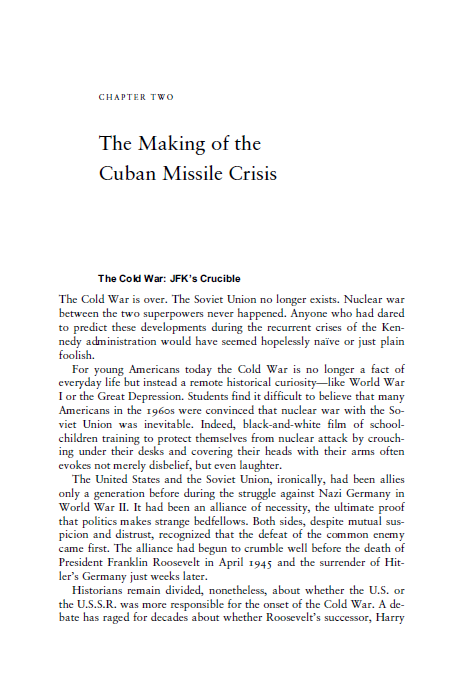
\includegraphics[width=0.48\textwidth]{./chapters/chapter51a.png}}
\caption{Style 51 Spread.}
\end{figure}

\section{Some notes}

If you observe this style carefully you will notice that the full title block, including the epigraph are set in from the left margin. This is achieved by setting appropriate \cs{hspace} lengths. The epigraph key width, needs to have the right distance and calculate the width. Example~ \ref{ch:style51} demonstrates the technique.

\cxset{chapter opening=anywhere}

\example
\begin{verbatim}
\cxset{style51,
   chapter opening=anywhere,
   epigraph align=right,
   epigraph width=\dimexpr(\textwidth-1.0cm)\relax,
  }
\end{verbatim}

\solution
    
\chapter{Introduction to Chapter Style 51}
\epigraph{\textbf{\sffamily Tuesday, October 16, 11:50 \textsc{a.m}, Cabinet Room}\par
               ``How do you know this is a medium-range ballistic missile?''}{President John F. Kennedy}
\lorem

\cxset{chapter opening=any,}

